\chapter{Methodology}

\section{Research Design}
\label{sec:meth:research_design}
This study uses an experimental pipeline development design in which an \gls{llm}-based biomedical information extraction system is developed iteratively against a fixed benchmark corpus before being frozen and evaluated on independently sampled, contemporary biomedical literature. The study consists of four main stages: development of the extraction pipeline against BioRED, selection of a pipeline iteration, evaluation of the chosen iteration, and construction and evaluation of a knowledge graph from the resulting contemporary extractions.

The main methodological idea of this design was the separation between development and evaluation. BioRED served as a basis for training, development, and test splits where this project's iterative pipeline development, made up of a set of Extraction Pipeline Iterations (\glspl{epi}), was conducted solely against the training and development splits. Each \gls{epi}'s prompt design and configuration was based on the previous \gls{epi}'s performance and optional further error analysis --- this approach began with an initial configuration (EPI 001), discussed further in Section~\ref{sec:meth:pipeline_development}, that established a baseline extraction pipeline using generic biomedical extraction instructions without BioRED-specific schema guidance. Pipeline development continued against the BioRED training split until performance plateaued, at which point the \gls{epi} configurations were frozen and no further prompt refinement or schema adjustment was performed. The frozen iterations were then evaluated against the BioRED development split, where their performance was compared with one another and the best performing \gls{epi} was selected. This distinction allows subsequent evaluation to be treated as a measure of the pipeline's performance, rather than further development.

The final \gls{epi} was then evaluated under two distinct stages. The first is benchmark evaluation, which measures the final \gls{epi}'s extraction performance against BiORED's held-out ground truth, establishing its performance within the distribution it was developed on. The second stage was generalisation evaluation, which applies the same pipeline to an independently assembled corpus of contemporary PubMed literature that the pipeline was not iteratively developed on. As the pipeline was not adapted to perform specifically on the contemporary corpus, any significant degradation in performance between them can be investigated as evidence of reduced generalisation to the contemporary corpus. Following extraction and normalisation on the contemporary corpus, the extracted entities and relations were assembled into a \gls{kg}.

\section{Datasets}
\label{sec:meth:datasets}

\subsection{BioRED Benchmark Corpus}
\label{subsec:meth:biored_benchmark_corpus}
The original BioRED corpus, as described in Section~\ref{subsec:lit:biored}, was used as the benchmark corpus for extraction pipeline development and evaluation in this project. The corpus consists of 600 manually annotated PubMed abstracts, assembled and released by the \gls{ncbi} and was obtained directly from the dataset's public GitHub repository. The BioRED-BC8 extension was also considered as it provides a more recent expert-annotated evaluation set: however, the original BioRED corpus was retained as the controlled benchmark as the study separately evaluates generalisation using literature independently retrieved through the PubMed \gls{api}, better reflecting the intended deployment pathway. BioRED-BC8 therefore represents a valuable alternative external evaluation dataset for future work.

The original version of the BioRED dataset divides 600 abstracts into a training split of 400 abstracts, a development split of 100 abstracts, and a test split of 100 abstracts. Each split was used for a distinct role in this study. The training split was used throughout iterative \gls{epi} development, providing the abstracts observed by the \gls{llm} in which all \gls{epi} configurations were developed on, the development split was then used to evaluate all frozen \gls{epi} configurations against one another, and the test spit was used exclusively for the final benchmark evaluation of the best-performing pipeline configuration and played no role in either pipeline development or \gls{epi} selection.

For each abstract, this project used the associated \gls{pmid}, title, and abstract text as the input passed to the extraction pipeline, together with the corresponding gold-standard annotations used as ground truth. These annotations consisted of each entity's type and text span and each relation's type. The following table summarises how each component of the BioRED dataset was used in this study:

\begin{table}[H]
    \centering
    \caption{BioRED Split Summary}
    \label{tab:biored_split_summary}
    \begin{tabularx}{\textwidth}{l Y Y Y}
        \toprule
        BioRED Component & No. of Abstracts & Purpose \\
        \midrule
        Training spit & 400 & EPI development and performance estimate \\
        Development split & 100 & EPI selection (held-out within BioRED) \\
        Test split & 100 & Final benchmark evaluation \\
        \bottomrule
    \end{tabularx}
\end{table}

It should be noted that \gls{epi} refinement was conducted using a fixed 35-abstract subsample of the BioRED training split, with each final \gls{epi} then evaluated across the full 400-abstract training split. Section~\pref \ discusses this methodological decision further.

BioRED's train, development, and test splits were each retrieved from the official BioRED GitHub repository as separate BioC-XML files. This process is discussed in Section~\ref{subsec:meth:data_preparation}.

\subsection{Contemporary Biomedical Corpus}
\label{subsec:meth:contemporary_biomedical_corpus}
An independently-assembled corpus of contemporary biomedical PubMed abstracts was constructed as the external evaluation set used to investigate generalisation to out-of-distribution data, as mentioned in Section~\ref{sec:lit:generalisation_to_contemporary_biomed_lit}. This \gls{cbc} included abstracts from papers published across 2024, 2025, and 2026 making up 282 total abstracts after duplication removal by \gls{pmid} and removal of entries with missing abstract texts. It should be explicitly noted that this corpus was assembled entirely independently of BioRED and played no role in \gls{epi} development or selection.

"Contemporary biomedical literature" was defined through a fixed set of either PubMed research queries, designed to give broad coverage of the wider field of general biomedicine, rather than a single subdomain. Four of the eight related to individual biomedical entity categories, generally mirroring BioRED's own entity type (gene/protein, disease/disorder, drug/chemical, and variant/mutation), while the remaining four combined two entity categories within a single query (gene and disease, drug and disease, gene and drug, variant and disease). This query configuration was chosen to feasibly maximise the likelihood of retrieving abstracts that include entity relationships, rather than only single entity mentions. Each of the eight queries were combined with a publication year filter for all three publication years, giving 24 distinct query-year combinations with 15 articles requested per combination. The table below summarises each query category and associated term.

\begin{table}[H]
    \centering
    \caption{Contemporary Biomedical Corpus Retrieval Query Summary}
    \label{tab:contemporary_corpus_query_summary}
    \begin{tabularx}{\textwidth}{l l}
        \toprule
        Query category & Query terms \\
        \midrule
        Gene/protein entity mention & \verb|"gene" OR "protein"| \\
        Disease/disorder entity mention & \verb|"disease" OR "disorder"| \\
        Drug/chemical entity mention & \verb|"drug" OR "chemical"| \\
        Variant/mutation entity mention & \verb|"variant" OR "mutation"| \\
        Gene-disease relation & \verb|"gene" AND "disease"| \\
        Drug-disease relation & \verb|"drug" AND "disease"| \\
        Gene-drug relation & \verb|"gene" AND "drug"| \\
        Variant-disease relation & \verb|"variant" AND "disease"| \\
        \bottomrule
    \end{tabularx}
\end{table}

Abstracts were retrieved from PubMed using the \gls{ncbi} Entrez E-utilities, accessed through Biopython's \verb|Bio.Entrez| module under a registered email address, as required by \gls{ncbi}'s usage policy. For each of the 24 query-year combinations an \verb|esearch| request was used to return 15 matching \glspl{pmid}, article title, abstract text, journal title, and publication year were extracted. Author names, \glspl{doi}, and keywords were not stored.

Across all query-year combinations, up to 360 records were requested in total: 15 results per query-year combination. After consolidating all returned results, duplicates were removed where \glspl{pmid} matched, along with any records with absent abstract text, leaving a final corpus of 282 abstracts. Beyond publication year, no sampling constraints were applied at this stage. A subset of the \gls{cbc} was selected for manual annotation, in order to provide ground-truth entity and relation labels which the frozen extraction pipeline could be evaluated against. This subset comprised 50 randomly sampled abstracts from the 282 total entries. The annotation procedure and resulting metrics are discussed in Section~\ref{subsec:meth:generalisation_evaluation}.

\subsection{Data Preparation}
\label{subsec:meth:data_preparation}
Although BioRED and the \gls{cbc} were retrieved from different sources and through different processes, both required conversion into a structured, tabular representation before use by the rest of the pipeline. \verb|pandas| DataFrames were used for both datasets, allowing later extraction and evaluation to be conducted easily over a tabular data, regardless of which dataset was used. BioRED was retrieved as raw BioC-XML and was parsed directly using \verb|xmltodict|, whereas the \gls{cbc} was retrieved via Biopython's \verb|Bio.Entrez| module, which returns PubMed records already parsed into Python dictionaries, requiring no further XML-parsing step.

For BioRED, each of the three split's files was parsed with \verb|xmltodict| into a Python dictionary before being converted into three separate \verb|pandas| DataFrames per split: a DataFrame containing each abstract's \gls{pmid}, title, and abstract text, an entity DataFrame containing one row per annotated entity mention, including its text span, entity type, and normalised identifier, and finally an entity relation DataFrame containing one row per annotated entity relation, including normalised identifiers of the two entities and their relation type.

For the \gls{cbc}, the entire returned dictionary was iterated over to extract each paper's \gls{pmid}, title, abstract text, and publication year. Where a paper had its abstract split into multiple segments, all segments were concatenated into a single string and duplicate records.

Relatively little additional preprocessing was conducted beyond this stage. For BioRED, no records were excluded during parsing and for the \gls{cbc}, no records were excluded beyond removal of duplicates and papers that had missing abstracts. For both corpora, all abstracts and corresponding title text string remained untouched as retrieved as the extraction pipeline provides abstract and title text directly to the \gls{llm} as natural language, rather than preprocessed text. The output of this stage was therefore a set of standardised, pipeline-ready CSV files.

\section{System Architecture}
\label{sec:meth:system_architecture}

The processed datasets discussed in Section~\ref{subsec:meth:data_preparation} formed the inputs to the extraction stage of the system. For BioRED, the resulting extractions were used for benchmark evaluation, whereas \gls{cbc} predictions were subsequently passed through normalisation, validation, and \gls{kg} construction. For each abstract, its title and text were passed to an \gls{llm}-based extraction step, which performed \gls{ner} and \gls{re} jointly rather than as separate \gls{llm} \gls{api} calls, returning structured entity and relation predictions. These predictions were parsed into the same tabular format used for BioRED's own annotations, allowing predicted and ground-truth extractions to be compared directly for subsequent evaluation. Figure~\pref \ below summarises this data flow across the implemented pipeline architecture.

% UPDATE THIS PARAGRAPH:
% "It says SapBERT embeds the mention and retrieves its nearest neighbour from “UMLS concept vector embeddings”. If you're now doing UMLS API candidate retrieval → SapBERT reranking of those candidates, that paragraph will need updating once you've actually implemented 4.6. This is important, but there is no reason to fix it before writing 4.5."
Extracted entity mentions then underwent entity normalisation, mapping each mention to its corresponding \gls{cui} in the \gls{umls}, using SapBERT \cite{liu2021sapbert} to encode each mention and retrieve its nearest neighbour among \gls{umls} concept vector embeddings by cosine similarity, before undergoing ontology-based validation, described in Section~\ref{subsec:meth:ontology_based_validation}. The resulting normalised, validated entities and relations were subsequently converted into nodes and edges and assembled into the final \gls{kg}.

The same extraction architecture was used across both BioRED and the \gls{cbc}, differing only in the input data supplied and presence of gold-standard annotations, with BioRED additionally providing ground truth against which extraction-level performance could be measured, and the \gls{cbc} providing only a manually annotated subset for this purpose, as described in Section~\ref{subsec:meth:contemporary_biomedical_corpus}. Although the pipeline's specific configuration changed across the \gls{epi} development process, the overall architecture described above remained consistent throughout.

\begin{figure}[H]
    \centering
    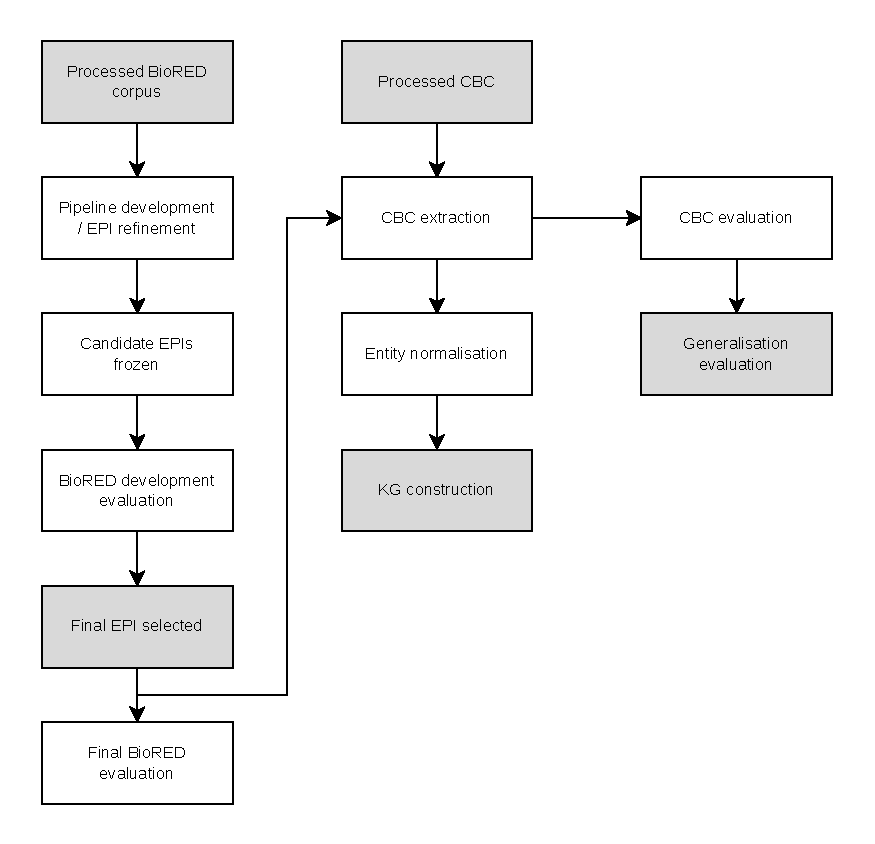
\includegraphics[width=\textwidth]{../img/system_architecture.pdf}
    \caption{System architecture and data flow, from prepared corpus input through extraction, normalisation, and \gls{kg} construction, to the three evaluation branches described in Section~\ref{sec:meth:evaluation}. Grey shading highlights key inputs, final stages, and outputs.}
    \label{fig:system_architecture}
\end{figure}

\section{Information Extraction Pipeline}
\label{sec:meth:info_extraction_pipeline}
Prepared title and abstract text produced in Section~\ref{subsec:meth:data_preparation}, was used as the input to a pretrained \gls{llm} accessed through an \gls{api}. \gls{ner} and \gls{re} were performed together within a single \gls{api} request per abstract, with the model instructed to return entities and relationships following the BioRED extraction schema. The raw response was parsed into structured entity and relation predictions and stored for subsequent evaluation and processing.

\subsection{LLM Configuration}
\label{subsec:meth:llm_config}
All extraction was performed using a single model, OpenAI's \verb|gpt-5.6-luna|, accessed via the OpenAI Python \gls{sdk}'s Responses \gls{api} (\verb|client.responses.create|). This pretrained model was used, without any parameter fine-tuning, across every \gls{epi} configuration, ensuring that any performance difference observed across \glspl{epi} resulted from changes to the pipeline's prompt and extraction setup rather than a change in the model's configuration. Higher-cost models, geared more towards complex reasoning over budget-consciousness, were considered for this project, such as \verb|gpt-5.6-sol| or \verb|gpt-5.6-sol|, however, they were deemed infeasible for this project given the number of \gls{api} calls required across iterative \gls{epi} development and the full extraction runs on all four splits: the BioRED training, development and test splits, and the full \gls{cbc}. No additional generation parameters were set for temperature or generation seed as \verb|gpt-5.6-luna| did not allow either as a tuneable parameter to any of their reasoning models.

\verb|gpt-5.6-luna|'s reasoning effort parameter (\verb|reasoning| $\in$ \{\verb|low|, \verb|high|, \verb|medium|\}), controlling the magnitude of internal reasoning before a response output, was also left at its default setting throughout this project, rather than being specifically tuned. Unlike model temperature, this was not a constraint of the model, but a deliberate choice made without deeper investigation into its effect on extraction quality and reasoning effort was not treated as a variable between \glspl{epi}. Increasing reasoning effort typically increases both time and cost demand per request, and investigating its effect on extraction precision, recall, and consistency was concluded to be out of the scope given the time and budget constraints discussed in Section~\ref{sec:meth:cost_analysis}. This parameter is one that a larger-budget project with longer timeframe allowance could reasonably investigate.

However, the absence of a temperature parameter and omission of fine-tuned reasoning parameter has a direct methodological consequence. Without these parameters, the model's output for a given prompt and abstract is not guaranteed to be identical across repeated calls, even when all else remains constant. This results in two distinct sub-consequences: firstly, as the reproducibility of an \gls{epi}'s outputs across multiple identical calls is not guaranteed, any \gls{epi} that reuses its previous \gls{epi}'s prompt reuses its stored outputs, rather than calling the model again. Secondly, an observed change in extraction performance between two \gls{epi}s using different prompt or extraction pipeline configurations cannot be attributed with complete certainty to the \gls{epi} refinement alone, as variation in performance may reflect natural variation in the model's generation, rather than just the effects of the update. This is partially mitigated by the fact that each \gls{epi} during the development stage was evaluated across the full BioRED training split ($n = 400$), rather than a small subsample of abstracts, which reduces the effects of variability of individual responses on performance metrics. Table \ref{tab:extraction_model_config_summary} summarises the chosen model's extraction pipeline configuration.

\begin{table}[H]
    \centering
    \caption{Extraction Model Configuration Summary}
    \label{tab:extraction_model_config_summary}
    \begin{tabularx}{\textwidth}{l l}
        \toprule
        Parameter & Value \\
        \midrule
        Model & \verb|gpt-5.6-luna| \\
        Provider / \gls{sdk} & OpenAI Python \gls{sdk}, Responses \gls{api} \\
        Fine-tuning & None \\
        Temperature & Default (not explicitly set) \\
        Reasoning & Default (not explicitly set) \\
        Maximum output tokens & Default (not explicitly set) \\
        Generation seed &  Default (not explicitly set) \\
        Request timeout & 120s \\
        Maximum automatic retries & 2 \\
        Same model used across all \glspl{epi} & Yes \\
        \bottomrule
    \end{tabularx}
\end{table}

\subsection{Prompt and Extraction Schema}
\label{subsec:meth:prompt_and_extraction_schema}
\gls{epi} configurations were stored in externally from the project's main Python code as a set of dictionaries in JSON format including the \gls{epi}'s name, prompt version --- also stored externally in a prompt configuration JSON file: rather than embedding text directly into the extraction code, evaluation version --- discussed in Section~\ref{subsec:meth:structured_output_and_parsing}, and additional notes.

The prompt used by the project's \glspl{epi} was structured around several main components: a task definition instructing the model to extract entities and relationships exactly as they would be annotated under the official BioRED annotation guidelines, the BioRED guidelines themselves \cite{luo2022_biored}, an explicit list of the allowed entity and relationship types, evidence requirements, few-shot examples, and explicit output format instructions specifying the required JSON output. Each prompt version sequentially introduced one or more new components, initialised with the baseline prompt, including only explicit general instructions of the extraction task and the structured JSON output.

The permitted entity and relation types instructed in the prompt corresponded exactly to BioRED's own schema, given in Table~\ref{tab:permitted_entity_and_relation_types}.

The official BioRED annotation guidelines \cite{luo2022_biored}, retrieved from the corpus's public GitHub repository in PDF form, provides information of the corpus's own construction that are not relevant to instructing an \gls{llm}'s extraction, such as the corpus's data sampling methodology, tools used in its ground truth construction, and its full reference list. Before incorporating the guidelines into the prompt, the document was therefore condensed to contain only the entity and relation annotation rules relevant to the extraction task itself. No semantic content within the filtered guidelines was altered --- only its structure was changed, converting the document's bullet formatting into a consistently headed, nested bullet-point structure intended to be more easily parsed by the \gls{llm} when called. This condensed guideline version was stored in \texttt{.txt} format and embedded directly into the prompt as \texttt{\{biored\_ext\_guidelines\}}. The complete filtered BioRED extraction guidelines are provided in Appendix~\ref{app:filtered_biored_guidelines}.

\begin{table}[H]
    \centering
    \caption{Permitted Entity and Relation Types}
    \label{tab:permitted_entity_and_relation_types}
    \begin{tabularx}{\textwidth}{l l}
        \toprule
        Entity types & Relation Types \\
        \midrule
        ChemicalEntity & Association \\
        DiseaseOrPhenotypic Feature & Bind \\
        GeneOrGeneProduct & Comparison \\
        SequenceVariant & Conversion \\
        OrganismTaxon & Cotreatment \\
        CellLine & Drug\_Interaction \\
         & Negative\_Correlation \\
         & Positive\_Correlation \\
        \bottomrule
    \end{tabularx}
\end{table}

The evidence requirements instructed the model to base extractions only on information explicitly supported by the given abstract to avoid inferring entities or relationships from background biomedical knowledge rather than the abstract text itself, to avoid treating multiple entity mentions in the same sentence or context as automatically associated, and to avoid inferring a more specific relation type such as \verb|Positive_Correlation| or \verb|Negative_Correlation| than what the text explicitly included. The model was also instructed to exclude a relationship where it was uncertain if it satisfied these criteria. For each entity, the model was required to return its text and entity type, and for each relationship triple, two entities and a relation type.

Few-shot examples constructed directly from BioRED's own training split ground truth annotations, with each example including an abstract's text and its correct entity and relationship annotations in the same JSON structure the model was instructed to output. Three constant few-shot examples were included in each prompt by default. Once generated in its first inclusion in a prompt, the few shot block was exported and stored for subsequent inclusion, sharing the same configuration, rather than being resampled on every execution.

\subsection{Structured Output and Parsing}
\label{subsec:meth:structured_output_and_parsing}
The \gls{llm} was instructed through the prompt to return its extractions as a single JSON object containing two top-level keys: \texttt{entities} and \texttt{relationships}, each a list of extractions. No \gls{api}-level constraint existed to enforce this structure, how closely the outputs adhered to the specified JSON output depended entirely on how well the model followed the prompt's explicit instructions.

Each abstract's raw response text was parsed as JSON in Python. Where a response failed to parse from JSON-structured string to valid JSON, this was recorded as a parse failure and the abstract was treated as having produced no entities and no relationships, rather than causing the run to fail. No further validation, such as checking that returned entity or relation types belonged to the allowed schema, was conducted beyond this JSON-validity check. Successfully parsed entities and relationships were converted into tuples following the form \texttt{(PMID, entity text, type)} for entities and \texttt{(PMID, entity 1, relation, entity 2)} for relationships. Entity text was stripped of any excess whitespace and stored in lowercase. These predictions sets were then converted into the same tabular structure used for BiORED's own ground-truth entities and relations, described in Section~\ref{subsec:meth:data_preparation}, allowing predicted and ground-truth extractions to be compared directly during evaluation.

Finally, after each \gls{epi}'s final extraction run on the entire BioRED train set, the run was exported as its own run in full, storing the \gls{epi}'s identifier (e.g.: \texttt{epi\_001}), the dataset split it was evaluated on, the prompt and evaluation version used, the number of abstracts processed, the count of failed JSON parses, the raw prompt template, each abstract's raw total model output, the parsed entity and relation predictions, and the evaluation metrics and errors resulting from that run. The raw and parsed extractions were stored as, as previously mentioned, when a new \gls{epi} reused the previous \gls{epi}'s prompt version and only updated the evaluation approach, the previous \gls{epi}'s outputs were used --- storing outputs allowed for the importing of previous \gls{epi} outputs when necessary. How these logged runs were compared and used to select a final \gls{epi} is described in Section~\ref{sec:meth:pipeline_development}. The complete text of each prompt version is provided in Appendix~\ref{app:extraction_prompts}.

\section{Pipeline Development}
\label{sec:meth:pipeline_development}
Development of the extraction pipeline was organised as a sequence of Extraction Pipeline Iterations \glspl{epi}. Each \gls{epi} represented a pre-configured combination of a prompt version and evaluation version and was assigned a unique identifier (e.g., \texttt{epi\_001}) used to track it during development. Changes between \glspl{epi} were introduced incrementally, with each new \gls{epi} modifying one or a few components of the previous iteration, so that the effect of an individual methodological change could be isolated, rather than observing the effects of several significant changes. As described in Section~\ref{sec:meth:research_design}, all \gls{epi} development and refinement was conducted exclusively against the BioRED training split, with the BioRED development split used for the comparison of candidate \glspl{epi}, playing no role in extraction pipeline refinement. Each \gls{epi}'s full configuration, prompt template, and extraction outputs were automatically logged after extraction, allowing outputs to be reused directly by a subsequent \gls{epi} where prompt version remained unchanged between them.

\subsection{Extraction Pipeline Iterations}
\label{subsec:meth:extraction_pipeline_iterations}
Table~\ref{tab:epi_summary} summarises the configuration of all \glspl{epi} produced during development, including the main methodological change in addition to the previous iteration.

\begin{table}[H]
    \centering
    \caption{Extraction Pipeline Iteration summary}
    \label{tab:epi_summary}
    \begin{tabularx}{\textwidth}{@{} l p{2.4cm} p{4.0cm} X @{}}
        \toprule
        EPI & Prompt & Evaluation & Main addition/purpose \\
        \midrule
        \texttt{epi\_001} & \texttt{v1} & \texttt{v1} (strict matching) & Baseline configuration \\
        \texttt{epi\_002} & \texttt{v1} & \texttt{v2} (relaxed matching) & Relaxed matching to baseline prompt \\
        \texttt{epi\_003} & \texttt{v2} & \texttt{v2} & Filtered BioRED guidelines and allowed entity and relation types \\
        \texttt{epi\_004} & \texttt{v2} & \texttt{v3} (cosine matching) & Cosine matching \\
        \texttt{epi\_005} & \texttt{v3} & \texttt{v3} (cosine matching) & Few-shot examples \\
        \texttt{epi\_006} & \texttt{v3} & \texttt{v4} (relation order invariance) & Relation order invariant evaluation \\
        \texttt{epi\_007} & \texttt{v4} & \texttt{v4} & Targeted suppression of background biomedical knowledge \\
        \texttt{epi\_008} & \texttt{v5} & \texttt{v4} & Explicit instructions preventing inference of an unsupported extraction \\
        \texttt{epi\_009} & \texttt{v6} & \texttt{v4} & Explicit precision-over-recall instructions \\
        \texttt{epi\_010} & \texttt{v7} & \texttt{v4} & Precision-focussed conservative extraction instructions \\
        \texttt{epi\_011} & \texttt{v8} & \texttt{v4} & Targeted suppression of excessive relation over-extraction \\
        \bottomrule
    \end{tabularx}
\end{table}

Together, this sequence of pipeline iterations reflects several broad stages of development, rather than a linear progression of independent changes: an initial baseline extraction stage (\texttt{epi\_001}-\texttt{002}), alignment of the prompt with BioRED's own entity and relation schema (\texttt{epi\_003}-\texttt{004}), introduction of few-shot prompting (\texttt{epi\_005}), concurrent evaluation logic progression (\texttt{epi\_001}--\texttt{006}), tightening of evidence requirements (\texttt{epi\_007}--\texttt{008}), and a final stage of prompt refinement targeting over-extraction (\texttt{epi\_009}--\texttt{011}). It should be noted that, for each \gls{epi} where evaluation methodology was updated, the previous \gls{epi}'s prompt outputs were used. This allowed direct analysis of the evaluation refinement's effects on extraction performance metrics.

As mentioned above, evaluation methodology applied to each \gls{epi}'s outputs also evolve over the course of development, concurrently with prompt refinement. As summarised in Table~\ref{tab:epi_summary}, the baseline \gls{epi} was assessed using strict matching, where only exact string matching between an extraction and a ground-truth counted as a success. Manual inspection of errors --- automatically recorded in each \gls{epi}'s stored log, including \glspl{fp} and \glspl{fn} --- indicated that numerous extractions represented the correct biomedical concept, yet differed from the ground-truth annotation in span boundary or string representation, meaning strict matching classified some semantically correct predictions as errors. This motivated the introduction of relaxed matching, which allowed correct-match classification where the string representation of the extracted entity differed slightly from that of its corresponding ground truth. However, this implementation was found to be insufficient where an extraction and its ground truth were semantically equivalent but expressed using disparate string representations, exceeding solely a mismatch between entity name boundaries. As a result, subsequent cosine-similarity-based matching was introduced, which compared the vector embeddings of extracted and ground truth entity mentions using a fixed threshold. The exact configuration and implementation of strict, relaxed, cosine, and relation order invariance evaluation approaches are described in Section~\ref{sec:meth:evaluation}.

% Put in Sec. 4.7
% Embeddings were generated using \texttt{S-PubMedBert-MS-MARCO} \pref, a Sentence-BERT model pretrained on PubMed abstracts and fined tuned for semantic search on the Microsoft Machine Reading Comprehension (MS MARCO) dataset. This model was selected over general-purpose alternatives, such as OpenAI's \texttt{text-embedding-3-large}, as the fine-tuned, domain specific model was expected to produce more accurate representations of biomedical terminology, where subtle differences between distinct concepts are captured, where general-purpose embedding models are not trained to.

% For each extraction--ground truth comparison, cosine similarity was computed between embedding vectors, and a match was recorded where this similarity met or exceeded a pre-defined threshold of 0.85. Matching was performed in a greedy approach, where for each predicted mention, the highest-scoring unmatched ground truth mention was selected as a match and removed from evaluation of subsequent extractions. This prevented evaluation where a single ground truth annotation counted as a match for multiple extractions.

% Include strict, relaxed, and how relation order invariance applies to all evaluation methods for relations

% After analysis of initial cosine evaluation implemented in \texttt{epi\_005}'s extraction performance, errors indicated that a few relation extractions were marked as non-matches where the extracted relation's entities appeared in the opposite order of their corresponding ground truth. As a result, relation order invariance matching was introduced where both orders of a relationship triple's entities were evaluated, where a match of either order counted as a correct extraction for that extraction--ground truth pair:

% \vspace{0.75em}
% \newcommand{\triple}[3]{(\text{#1},\, \text{#2},\, \text{#3})}

% \noindent\textbf{Before relation order invariance:}
% \vspace{0.25em}
% \[
% \triple{warfarin}{Positive\_Correlation}{ICH}
% \;\neq\;
% \triple{ICH}{Positive\_Correlation}{warfarin}
% \]

% \noindent\textbf{After relation order invariance:}
% \vspace{0.25em}
% \[
% \triple{warfarin}{Positive\_Correlation}{ICH}
% \;\equiv\;
% \triple{ICH}{Positive\_Correlation}{warfarin}
% \]

When necessary, to understand the nature of extraction errors, false positive (\gls{fp}) and false negative (\gls{fn}) relation errors produced by the current \gls{epi} were sampled and analysed. This analysis was restricted to relations, rather than entities, as relation extraction exhibited significantly weaker performance throughout development and was therefore the main focus of this investigation. For the selected \gls{epi}, up to 50 false positive \gls{fp} and 50 false negative \gls{fn} errors were randomly sampled, using a fixed random seed for reproducibility, and assigned one of a set of pre-defined error categories.

Given the volume of errors sampled, manual assignment of each error to a pre-defined error category was not feasible. Instead, categorisation was performed automatically using the same \gls{llm} used for the extraction process. For each sampled error, the model was provided with the incorrect relation, the error type (\gls{fn} or \gls{fp}), the source abstract, and the corresponding BioRED ground truth relations for that abstract. The model was then instructed to assign the error to exactly one of seven predefined error categories (Table~\ref{tab:error_categories}), each including a description of the conditions of when the error category is true. The complete prompt supplied to the \gls{llm} during error analysis is provided in Appendix~\ref{app:sec:error_categorisation_prompt}.

\begin{table}[H]
    \centering
    \caption{Error category summary}
    \label{tab:error_categories}
    \begin{tabularx}{\textwidth}{l X}
        \toprule
        Category & Description \\
        \midrule
        Wrong relation type & "The correct entity pair is identified, but the predicted relation type differs from the BioRED ground truth." \\
        Duplicate/coreference & "The error results from duplicate entity mentions, abbreviations, aliases, or coreferential mentions of the same underlying entity." \\
        Unsupported relation & "The predicted relation is not supported by the abstract or BioRED annotation policy." \\
        Entity boundary/synonyms mismatch & "The prediction and ground truth refer to the same underlying entity, but differ in span, wording, abbreviation, or synonym representation." \\
        Missing relation & "A BioRED ground-truth relation is supported by the abstract but was not extracted by the system." \\
        Evaluation artefact & "The prediction is substantively compatible with the ground truth, but is counted as an error because of the evaluation or matching procedure." \\
        Other/unclear & "The primary cause cannot be confidently assigned to any other category." \\
        \bottomrule
    \end{tabularx}
\end{table}

These category distributions were used diagnostically, precision, recall, and F1 to establish whether an \gls{epi}'s performance reflected true extraction failure, evaluation artefacts, or specific prompt configuration issues. Analysis showed that unsupported relations was a significant false-positive category through much of development, directly motivating the evidence requirement prompt refinements in \texttt{epi\_007}--\texttt{epi\_011}. A significant proportion of false negatives were also categorised as evaluation artefacts, supporting the introduction of cosine-based matching. Figure~\ref{fig:epi_003_train_error_distribution} shows a representative error distribution figure from one stage of this analysis (\text{epi\_009}) --- the remaining error distribution figures are shown in Appendix~\ref{app:epi_error_dist_figures}.

\begin{figure}[H]
    \centering
    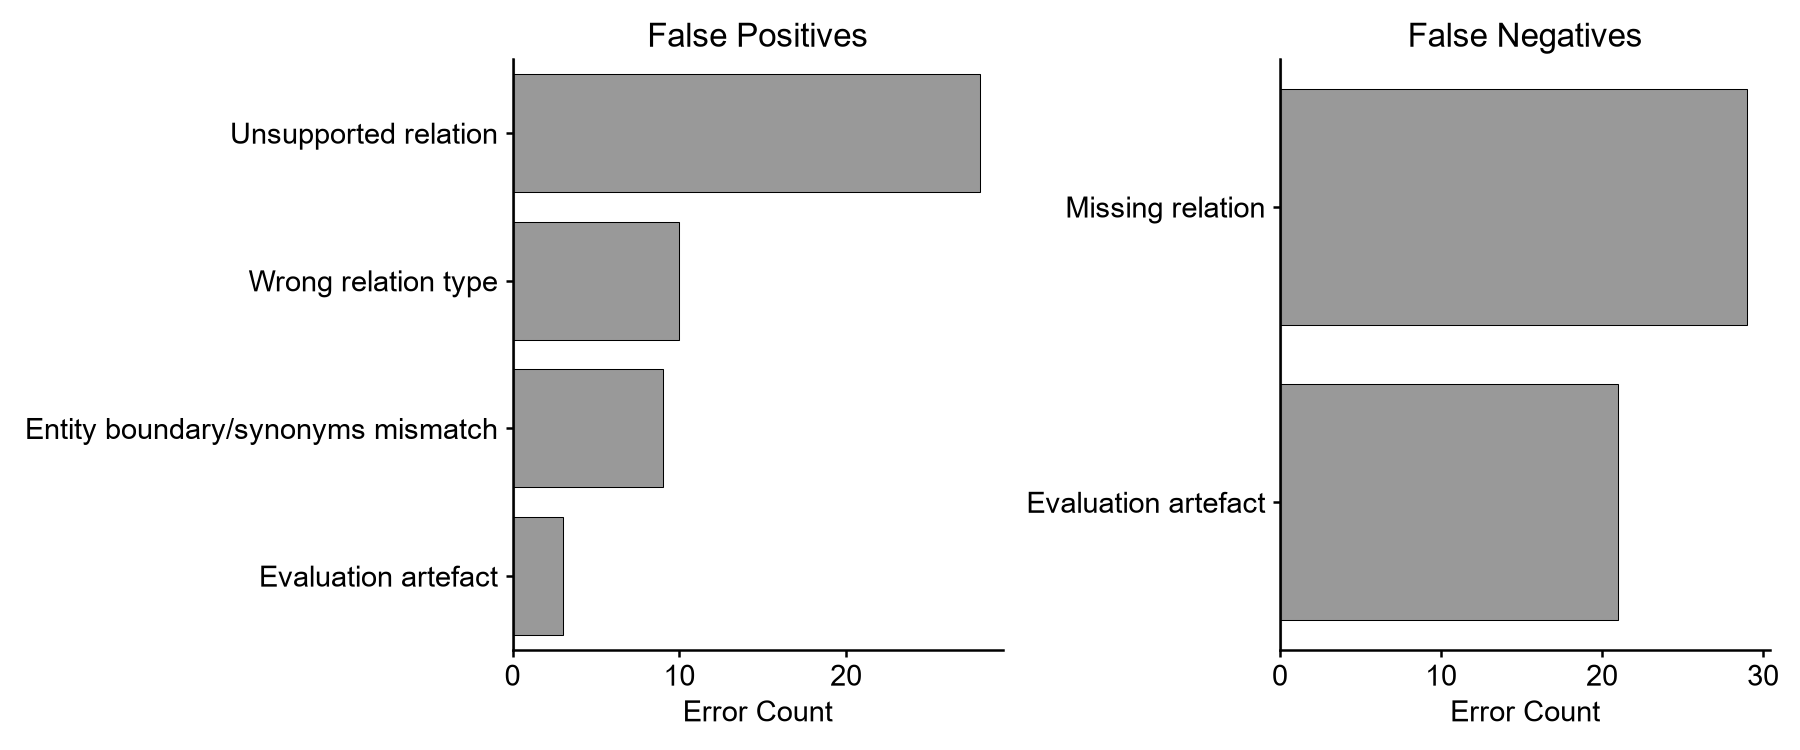
\includegraphics[width=1\textwidth]{../../../img/error_analysis/biored_train/epi_009.png}
    \caption{\texttt{epi\_003} relation error distribution.}
    \label{fig:epi_003_train_error_distribution}
\end{figure}

\subsection{Development and Model Selection}
\label{subsec:meth:development_and_model_selection}
Iterative \gls{epi} development against the BioRED training split contiued until further prompt or evaluation refinements produced only marginal changes in extraction performance metrics. At this point, all candidate \gls{epi} configurations were frozen and no further prompt or schema adjustment was made

Figure~\ref{fig:epi_performance} in Section~\pref \ shows the entity and relation precision, recall, and F1 across all \glspl{epi} measured on the BioRED development split, after being refined on the training split, allowing performance to be tracked across sequential extraction pipeline refinements. On the basis of primarily F1, and secondarily precision and recall, \texttt{epi\_007}, \texttt{epi\_008}, and \texttt{epi\_009} were selected for further comparison.

Figure~\ref{fig:top3_epi_relation_performance} (Section~\pref) compares these three selected \glspl{epi} directly on relation precision, recall, and F1, again, evaluated on the unseen BioRED development split. Final selection between the three candidates was mainly based on relation F1, as relation extraction was the main target of refinement at this stage of development. \texttt{epi\_009} was selected as it exhibited the highest F1 and precision, while narrowly underperforming compared to \texttt{epi\_007} on recall. It should be noted that while \texttt{epi\_009} marginally outperformed its competitors on balance, the differences in extraction performance for all three performance metrics were near negligible.

No further prompt, schema, or evaluation changes were made to the selected \gls{epi} following this comparison. The resulting configuration was therefore frozen and used without modification for the final BioRED benchmark evaluation and extraction of the \gls{cbc}.

\subsection{Final Pipeline}
\label{subsec:meth:final_pipeline}
The final extraction pipeline configuration selected through the process above is summarised in Table~\ref{tab:final_epi_config}

\begin{table}[H]
    \centering
    \caption{Final Extraction Pipeline Configuration}
    \label{tab:final_epi_config}
    \begin{tabularx}{\textwidth}{l X}
        \toprule
        Component & Final configuration \\
        \midrule
        \gls{epi} & \texttt{epi\_009} \\
        Prompt version & \texttt{v6} (Suppression of background knowledge, unsupported extraction inference suppression) \\
        Evaluation version & \texttt{v4} (Cosine-based, relation order invariant) \\
        \gls{llm} & \texttt{gpt-5.6-luna} \\
        Few-shot examples & 3 fixed BioRED training examples \\
        Entity schema & BioRED six entity types (Table~\ref{tab:permitted_entity_and_relation_types}) \\
        Relation schema & BioRED eight relation types (Table~\ref{tab:permitted_entity_and_relation_types}) \\
        Output format & JSON object \\
        \bottomrule
    \end{tabularx}
\end{table}

\section{Contemporary Knowledge Graph Construction}
\label{sec:meth:contemporary_kg_construction}

\subsection{Contemporary Corpus Extraction}
\label{subsec:meth:contemporary_corpus_extraction}

\subsection{Graph Construction}
\label{subsec:meth:graph_construction}

\subsection{Ontology-Based Validation}
\label{subsec:meth:ontology_based_validation}

\section{Evaluation}
\label{sec:meth:evaluation}

\subsection{Entity Evaluation}
\label{subsec:meth:entity_evaluation}

\subsection{Relation Evaluation}
\label{subsec:meth:relation_evaluation}

\subsection{Generalisation Evaluation}
\label{subsec:meth:generalisation_evaluation}

\subsection{Knowledge Graph Evaluation}
\label{subsec:meth:knowledge_graph_evaluation}

\section{Cost Analysis}
\label{sec:meth:cost_analysis}
